

	{\color{gray}Consider the problem of inserting the following keys, in the given order, into an empty B+-tree where nodes can hold up to 3 values:}
	
	{\color{gray}Parmesão, Ilha, Camembert, Fresco, Requeijão, Azeitão, Alverca, Serra, Alcobaça, Roquefort, Flamengo, Emmental, Évora, Creme, Serpa, Quark}

1 - Alcobaça

2 - Alverca

3 - Azeitão

4 - Camembert

5 - Creme

6 - Emmental

7 - Évora

8 - Flamengo

9 - Fresco

10 - Ilha

11 - Parmesão

12 - Quark

13 - Requeijão

14 - Roquefort

15 - Serpa

16 - Serra

	\subsection{}
	{\color{gray}Draw the tree after each insertion.}
 		Insertion order: 11, 10, 4, 9, 13, 3, 2, 16, 1, 14, 8, 6, 7, 5, 15, 12



\textbf{Insert 11 (Parmesão)}
\begin{center}

\begin{tikzpicture}
\tikzstyle{bplus}=[inner sep=0pt,font=\small]
\tikzstyle{every node}=[bplus]
\tikzstyle{level 1}=[sibling distance=15mm]
\tikzstyle{level 2}=[sibling distance=15mm]
\node {\onenode{\cellcolor{green}11}} [-]
;\end{tikzpicture}
\end{center}

\textbf{Insert 10 (Ilha)}
\begin{center}

\begin{tikzpicture}
\tikzstyle{bplus}=[inner sep=0pt,font=\small]
\tikzstyle{every node}=[bplus]
\tikzstyle{level 1}=[sibling distance=15mm]
\tikzstyle{level 2}=[sibling distance=15mm]
\node {\twonode{\cellcolor{green}10}{11}} [-]
;\end{tikzpicture}
\end{center}

\textbf{Insert 4 (Camembert)}
\begin{center}

\begin{tikzpicture}
\tikzstyle{bplus}=[inner sep=0pt,font=\small]
\tikzstyle{every node}=[bplus]
\tikzstyle{level 1}=[sibling distance=15mm]
\tikzstyle{level 2}=[sibling distance=15mm]
\node {\threenode{\cellcolor{green}4}{10}{11}} [-]
;
\end{tikzpicture}
\end{center}


\textbf{Insert 9 (Fresco)}

9 is inserted on leaf node [4,10,11], which will split into [4,9] and [10,11], 10 goes up.

\begin{center}
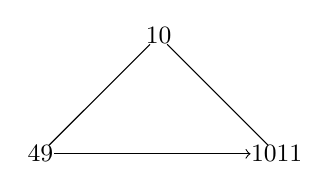
\begin{tikzpicture}
\tikzstyle{bplus}=[inner sep=0pt,font=\small]
\tikzstyle{every node}=[bplus]
\tikzstyle{level 1}=[sibling distance=30mm]
\tikzstyle{level 2}=[sibling distance=30mm]
\node {\onenode{\cellcolor{yellow}10}} [-]
  child {node (a) {\twonode{4}{\cellcolor{green}9}}}
  child {node (b) {\twonode{10}{11}}} 
;
\draw[->] (a) -- (b);
\end{tikzpicture}
\end{center}

\textbf{Insert 13 (Requeijão)}
\begin{center}
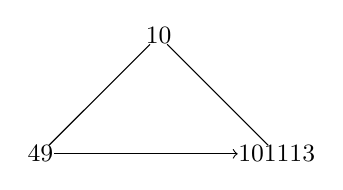
\begin{tikzpicture}
\tikzstyle{bplus}=[inner sep=0pt,font=\small]
\tikzstyle{every node}=[bplus]
\tikzstyle{level 1}=[sibling distance=30mm]
\tikzstyle{level 2}=[sibling distance=30mm]
\node {\onenode{10}} [-]
  child {node (a) {\twonode{4}{9}}}
  child {node (b) {\threenode{10}{11}{\cellcolor{green}13}}} 
;
\draw[->] (a) -- (b);
\end{tikzpicture}
\end{center}

\textbf{Insert 3 (Azeitão)}
\begin{center}
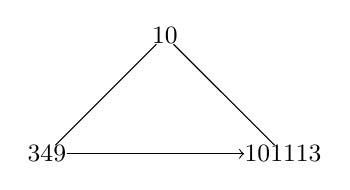
\begin{tikzpicture}
\tikzstyle{bplus}=[inner sep=0pt,font=\small]
\tikzstyle{every node}=[bplus]
\tikzstyle{level 1}=[sibling distance=30mm]
\tikzstyle{level 2}=[sibling distance=30mm]
\node {\onenode{10}} [-]
  child {node (a) {\threenode{\cellcolor{green}3}{4}{9}}}
  child {node (b) {\threenode{10}{11}{13}}} 
;
\draw[->] (a) -- (b);
\end{tikzpicture}
\end{center}

\textbf{Insert 2 (Alverca)}

2 is inserted on leaf node [3,4,9], which will split into [2,3] and [4,9], 4 goes up.

\begin{center}
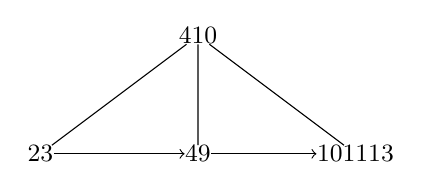
\begin{tikzpicture}
\tikzstyle{bplus}=[inner sep=0pt,font=\small]
\tikzstyle{every node}=[bplus]
\tikzstyle{level 1}=[sibling distance=20mm]
\tikzstyle{level 2}=[sibling distance=20mm]
\node {\twonode{\cellcolor{yellow}4}{10}} [-]
  child {node (a) {\twonode{\cellcolor{green}2}{3}}}
  child {node (b) {\twonode{4}{9}}}
  child {node (c) {\threenode{10}{11}{13}}} 
;
\draw[->] (a) -- (b);
\draw[->] (b) -- (c);
\end{tikzpicture}
\end{center}

\textbf{Insert 16 (Serra)}

16 is inserted on leaf node [10,11,13], which will split into [10,11] and [13,16], 13 goes up.

\begin{center}
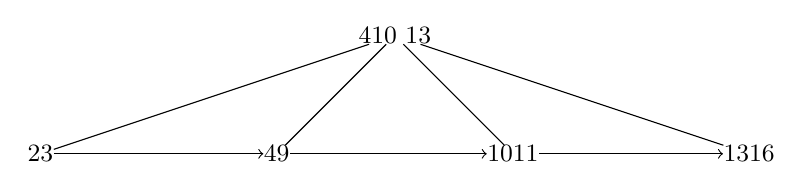
\begin{tikzpicture}
\tikzstyle{bplus}=[inner sep=0pt,font=\small]
\tikzstyle{every node}=[bplus]
\tikzstyle{level 1}=[sibling distance=30mm]
\tikzstyle{level 2}=[sibling distance=20mm]
\node {\threenode{4}{10}{\cellcolor{yellow} 13}} [-]
  child {node (a) {\twonode{2}{3}}}
  child {node (b) {\twonode{4}{9}}}
  child {node (c) {\twonode{10}{11}}}
  child {node (d) {\twonode{13}{\cellcolor{green}16}}}
;
\draw[->] (a) -- (b);
\draw[->] (b) -- (c);
\draw[->] (c) -- (d);
\end{tikzpicture}
\end{center}

\textbf{Insert 1 (Alcobaça)}

\begin{center}
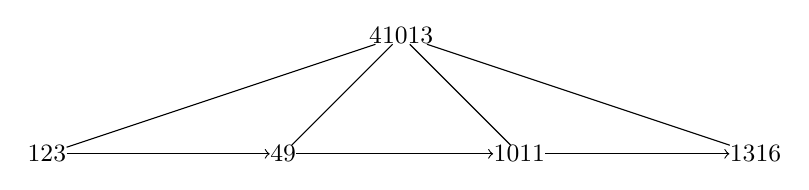
\begin{tikzpicture}
\tikzstyle{bplus}=[inner sep=0pt,font=\small]
\tikzstyle{every node}=[bplus]
\tikzstyle{level 1}=[sibling distance=30mm]
\tikzstyle{level 2}=[sibling distance=20mm]
\node {\threenode{4}{10}{13}} [-]
  child {node (a) {\threenode{\cellcolor{green}1}{2}{3}}}
  child {node (b) {\twonode{4}{9}}}
  child {node (c) {\twonode{10}{11}}}
  child {node (d) {\twonode{13}{16}}}
;
\draw[->] (a) -- (b);
\draw[->] (b) -- (c);
\draw[->] (c) -- (d);
\end{tikzpicture}
\end{center}

\textbf{Insert 14 (Roquefort)}
\begin{center}
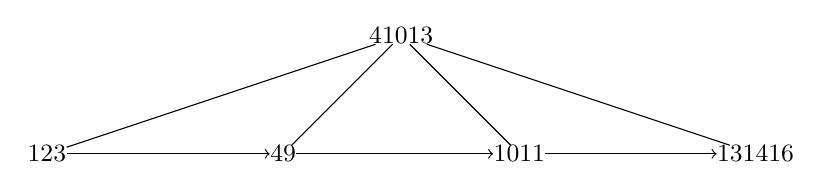
\begin{tikzpicture}
\tikzstyle{bplus}=[inner sep=0pt,font=\small]
\tikzstyle{every node}=[bplus]
\tikzstyle{level 1}=[sibling distance=30mm]
\tikzstyle{level 2}=[sibling distance=20mm]
\node {\threenode{4}{10}{13}} [-]
  child {node (a) {\threenode{1}{2}{3}}}
  child {node (b) {\twonode{4}{9}}}
  child {node (c) {\twonode{10}{11}}}
  child {node (d) {\threenode{13}{\cellcolor{green}14}{16}}}
;
\draw[->] (a) -- (b);
\draw[->] (b) -- (c);
\draw[->] (c) -- (d);
\end{tikzpicture}
\end{center}

\textbf{Insert 8 (Flamengo)}
\begin{center}
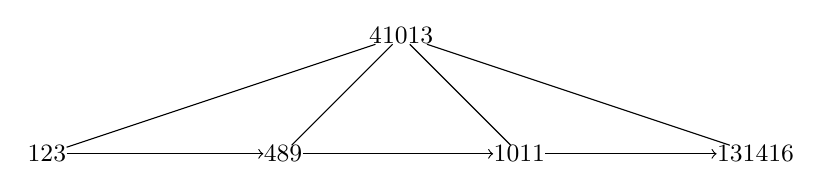
\begin{tikzpicture}
\tikzstyle{bplus}=[inner sep=0pt,font=\small]
\tikzstyle{every node}=[bplus]
\tikzstyle{level 1}=[sibling distance=30mm]
\tikzstyle{level 2}=[sibling distance=20mm]
\node {\threenode{4}{10}{13}} [-]
  child {node (a) {\threenode{1}{2}{3}}}
  child {node (b) {\threenode{4}{\cellcolor{green}8}{9}}}
  child {node (c) {\twonode{10}{11}}}
  child {node (d) {\threenode{13}{14}{16}}}
;
\draw[->] (a) -- (b);
\draw[->] (b) -- (c);
\draw[->] (c) -- (d);
\end{tikzpicture}
\end{center}

\textbf{Insert 6 (Emmental)}

6 is inserted on leaf node [4,8,9], which will split into [4,6] and [8,9], 8 goes up.

8 is inserted on non leaf node [4|10|13], which will split into [4] and [10|13], 8 goes up. [4] points to the original leaf node and [10|13] points to the new leaf node [8|9].

\begin{center}
\begin{tikzpicture}
\tikzstyle{bplus}=[inner sep=0pt,font=\small]
\tikzstyle{every node}=[bplus]
\tikzstyle{level 1}=[sibling distance=80mm]
\tikzstyle{level 2}=[sibling distance=25mm]
\tikzstyle{level 3}=[sibling distance=5mm]
\node {\onenode{\cellcolor{yellow}8}} [-]
  child {node {\onenode{4}}
    child {node (a) {\threenode{1}{2}{3}}}
    child {node (b) {\twonode{4}{\cellcolor{green}6}}}  
  }
  child {node {\twonode{10}{13}}
    child {node (c) {\twonode{8}{9}}}  
    child {node (d) {\twonode{10}{11}}}  
    child {node (e) {\threenode{13}{14}{16}}}
  }
;
\draw[->] (a) -- (b);
\draw[->] (b) -- (c);
\draw[->] (c) -- (d);
\draw[->] (d) -- (e);
\end{tikzpicture}
\end{center}


\textbf{Insert 7 (Évora)}
\begin{center}
\begin{tikzpicture}
\tikzstyle{bplus}=[inner sep=0pt,font=\small]
\tikzstyle{every node}=[bplus]
\tikzstyle{level 1}=[sibling distance=80mm]
\tikzstyle{level 2}=[sibling distance=25mm]
\tikzstyle{level 3}=[sibling distance=5mm]
\node {\onenode{8}} [-]
  child {node {\onenode{4}}
    child {node (a) {\threenode{1}{2}{3}}}
    child {node (b) {\threenode{4}{6}{\cellcolor{green}7}}}  
  }
  child {node {\twonode{10}{13}}
    child {node (c) {\twonode{8}{9}}}  
    child {node (d) {\twonode{10}{11}}}  
    child {node (e) {\threenode{13}{14}{16}}}
  }
;
\draw[->] (a) -- (b);
\draw[->] (b) -- (c);
\draw[->] (c) -- (d);
\draw[->] (d) -- (e);
\end{tikzpicture}
\end{center}

\textbf{Insert 5 (Creme)}

5 is inserted on leaf node [4,6,7], which will split into [4,5] and [6,7], 6 goes up.

\begin{center}
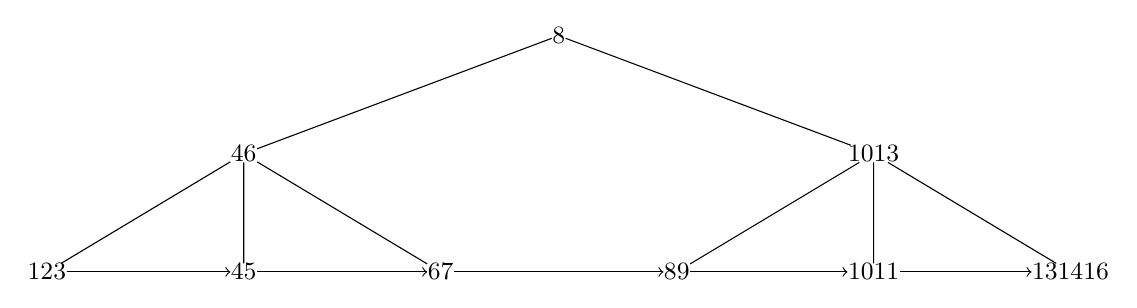
\begin{tikzpicture}
\tikzstyle{bplus}=[inner sep=0pt,font=\small]
\tikzstyle{every node}=[bplus]
\tikzstyle{level 1}=[sibling distance=80mm]
\tikzstyle{level 2}=[sibling distance=25mm]
\tikzstyle{level 3}=[sibling distance=5mm]
\node {\onenode{8}} [-]
  child {node {\twonode{4}{\cellcolor{yellow}6}}
    child {node (a) {\threenode{1}{2}{3}}}
    child {node (b) {\twonode{4}{\cellcolor{green}5}}}  
    child {node (c) {\twonode{6}{7}}}  
  }
  child {node {\twonode{10}{13}}
    child {node (d) {\twonode{8}{9}}}  
    child {node (e) {\twonode{10}{11}}}  
    child {node (f) {\threenode{13}{14}{16}}}
  }
;
\draw[->] (a) -- (b);
\draw[->] (b) -- (c);
\draw[->] (c) -- (d);
\draw[->] (d) -- (e);
\draw[->] (e) -- (f);
\end{tikzpicture}
\end{center}

\textbf{Insert 15 (Serpa)}

15 is inserted on leaf node [13,14,16], which will split into [13,14] and [15,16], 15 goes up.

\begin{center}
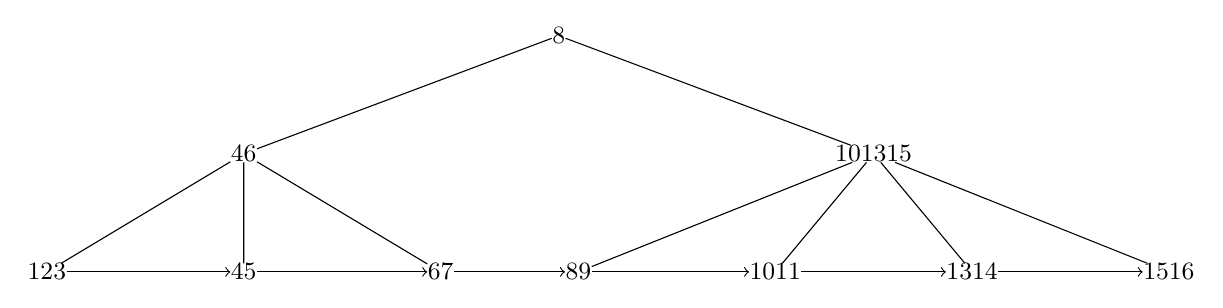
\begin{tikzpicture}
\tikzstyle{bplus}=[inner sep=0pt,font=\small]
\tikzstyle{every node}=[bplus]
\tikzstyle{level 1}=[sibling distance=80mm]
\tikzstyle{level 2}=[sibling distance=25mm]
\tikzstyle{level 3}=[sibling distance=5mm]

\node {\onenode{8}} [-]
  child {node {\twonode{4}{6}}
    child {node (a) {\threenode{1}{2}{3}}}
    child {node (b) {\twonode{4}{5}}}  
    child {node (c) {\twonode{6}{7}}}  
  }
  child {node {\threenode{10}{13}{\cellcolor{yellow}15}}
    child {node (d) {\twonode{8}{9}}}  
    child {node (e) {\twonode{10}{11}}}  
    child {node (f) {\twonode{13}{14}}}
    child {node (g) {\twonode{\cellcolor{green}15}{16}}}
  }
;
\draw[->] (a) -- (b);
\draw[->] (b) -- (c);
\draw[->] (c) -- (d);
\draw[->] (d) -- (e);
\draw[->] (e) -- (f);
\draw[->] (f) -- (g);
\end{tikzpicture}
\end{center}


\textbf{Insert 12 (Quark)}
\begin{center}
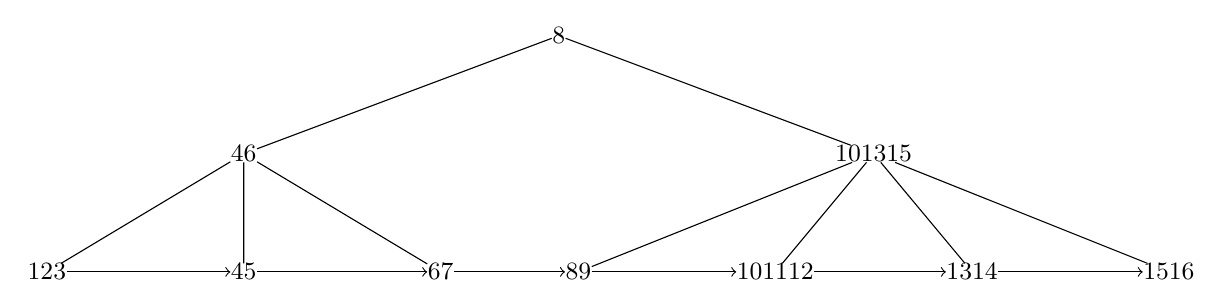
\begin{tikzpicture}
\tikzstyle{bplus}=[inner sep=0pt,font=\small]
\tikzstyle{every node}=[bplus]
\tikzstyle{level 1}=[sibling distance=80mm]
\tikzstyle{level 2}=[sibling distance=25mm]
\tikzstyle{level 3}=[sibling distance=5mm]

\node {\onenode{8}} [-]
  child {node {\twonode{4}{6}}
    child {node (a) {\threenode{1}{2}{3}}}
    child {node (b) {\twonode{4}{5}}}  
    child {node (c) {\twonode{6}{7}}}  
  }
  child {node {\threenode{10}{13}{15}}
    child {node (d) {\twonode{8}{9}}}  
    child {node (e) {\threenode{10}{11}{\cellcolor{green}12}}}  
    child {node (f) {\twonode{13}{14}}}
    child {node (g) {\twonode{15}{16}}}
  }
;
\draw[->] (a) -- (b);
\draw[->] (b) -- (c);
\draw[->] (c) -- (d);
\draw[->] (d) -- (e);
\draw[->] (e) -- (f);
\draw[->] (f) -- (g);
\end{tikzpicture}
\end{center}

	\subsection{}
	{\color{gray}Delete the following keys from the B+tree data structure from the previous exercise: Ilha; Flamengo; Emmental; Serpa. Draw the tree after each deletion.}

 		Deletion order: 10, 8, 6, 15

\textbf{Delete 10 (Ilha)}
\begin{center}
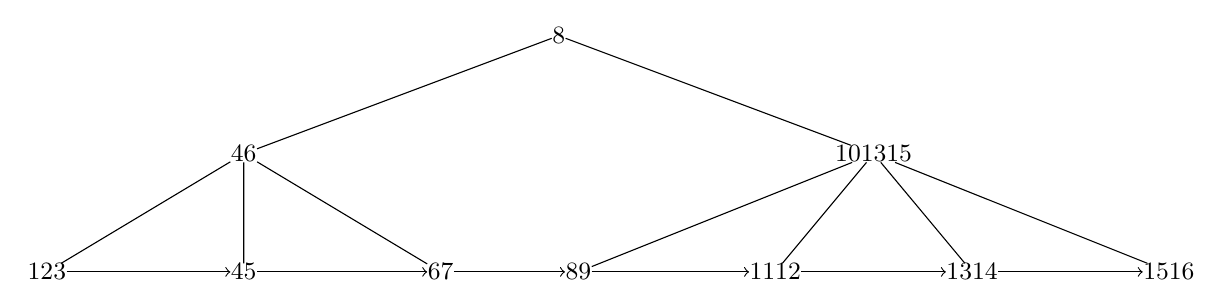
\begin{tikzpicture}
\tikzstyle{bplus}=[inner sep=0pt,font=\small]
\tikzstyle{every node}=[bplus]
\tikzstyle{level 1}=[sibling distance=80mm]
\tikzstyle{level 2}=[sibling distance=25mm]
\tikzstyle{level 3}=[sibling distance=5mm]

\node {\onenode{8}} [-]
  child {node {\twonode{4}{6}}
    child {node (a) {\threenode{1}{2}{3}}}
    child {node (b) {\twonode{4}{5}}}  
    child {node (c) {\twonode{6}{7}}}  
  }
  child {node {\threenode{10}{13}{15}}
    child {node (d) {\twonode{8}{9}}}  
    child {node (e) {\twonode{11}{12}}}  
    child {node (f) {\twonode{13}{14}}}
    child {node (g) {\twonode{15}{16}}}
  }
;
\draw[->] (a) -- (b);
\draw[->] (b) -- (c);
\draw[->] (c) -- (d);
\draw[->] (d) -- (e);
\draw[->] (e) -- (f);
\draw[->] (f) -- (g);
\end{tikzpicture}
\end{center}


\textbf{Delete 8 (Flamengo)}
\begin{center}
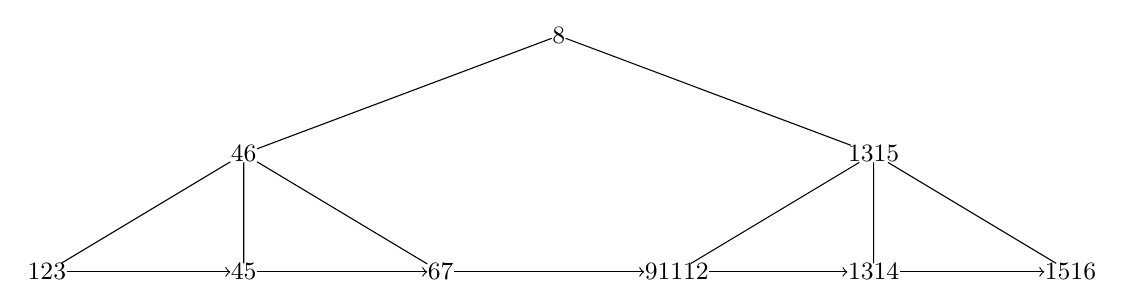
\begin{tikzpicture}
\tikzstyle{bplus}=[inner sep=0pt,font=\small]
\tikzstyle{every node}=[bplus]
\tikzstyle{level 1}=[sibling distance=80mm]
\tikzstyle{level 2}=[sibling distance=25mm]
\tikzstyle{level 3}=[sibling distance=5mm]

\node {\onenode{8}} [-]
  child {node {\twonode{4}{6}}
    child {node (a) {\threenode{1}{2}{3}}}
    child {node (b) {\twonode{4}{5}}}  
    child {node (c) {\twonode{6}{7}}}  
  }
  child {node {\twonode{13}{15}}
    child {node (d) {\threenode{9}{11}{12}}}    
    child {node (e) {\twonode{13}{14}}}
    child {node (f) {\twonode{15}{16}}}
  }
;
\draw[->] (a) -- (b);
\draw[->] (b) -- (c);
\draw[->] (c) -- (d);
\draw[->] (d) -- (e);
\draw[->] (e) -- (f);
\end{tikzpicture}
\end{center}

\textbf{Delete 6 (Emmental)}
\begin{center}
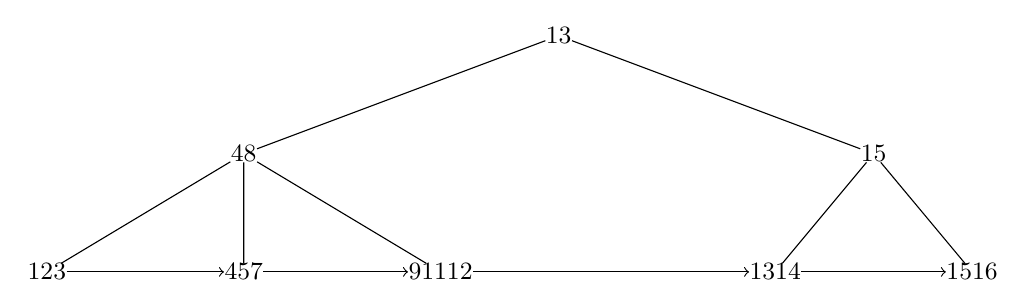
\begin{tikzpicture}
\tikzstyle{bplus}=[inner sep=0pt,font=\small]
\tikzstyle{every node}=[bplus]
\tikzstyle{level 1}=[sibling distance=80mm]
\tikzstyle{level 2}=[sibling distance=25mm]
\tikzstyle{level 3}=[sibling distance=5mm]

\node {\onenode{13}} [-]
  child {node {\twonode{4}{8}}
    child {node (a) {\threenode{1}{2}{3}}}
    child {node (b) {\threenode{4}{5}{7}}}  
    child {node (c) {\threenode{9}{11}{12}}}    
  }
  child {node {\onenode{15}}
    child {node (d) {\twonode{13}{14}}}
    child {node (e) {\twonode{15}{16}}}
  }
;
\draw[->] (a) -- (b);
\draw[->] (b) -- (c);
\draw[->] (c) -- (d);
\draw[->] (d) -- (e);
\end{tikzpicture}
\end{center}


\textbf{Delete 15 (Serpa)}
\begin{center}
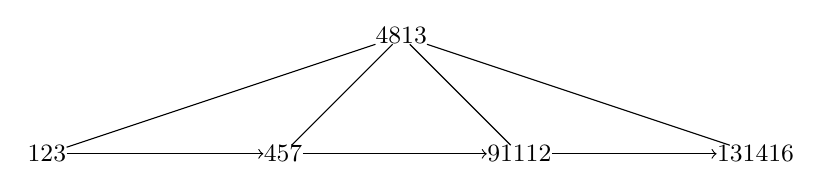
\begin{tikzpicture}
\tikzstyle{bplus}=[inner sep=0pt,font=\small]
\tikzstyle{every node}=[bplus]
\tikzstyle{level 1}=[sibling distance=30mm]
\tikzstyle{level 2}=[sibling distance=20mm]

\node {\threenode{4}{8}{13} } [-]
    child {node (a) {\threenode{1}{2}{3}}}
    child {node (b) {\threenode{4}{5}{7}}}  
    child {node (c) {\threenode{9}{11}{12}}}    
    child {node (d) {\threenode{13}{14}{16}}}
;
\draw[->] (a) -- (b);
\draw[->] (b) -- (c);
\draw[->] (c) -- (d);
\end{tikzpicture}
\end{center}


